\documentclass[../structure.tex]{subfiles}
\begin{document}
\chapter{Results}

\textbf{Outline}
\begin{itemize}
\item The device specification
\item Number of sample and description
\item Data source (from where we get it)
\item Number of points and tracts
\item The algorithm and method to compare with
\item Comparison :
\begin{itemize}
\item ISO MAP [to be discuss]
\item Time
\item Distance 
\item Visual
\end{itemize}
\end{itemize}

\begin{figure}[h!]
\centering
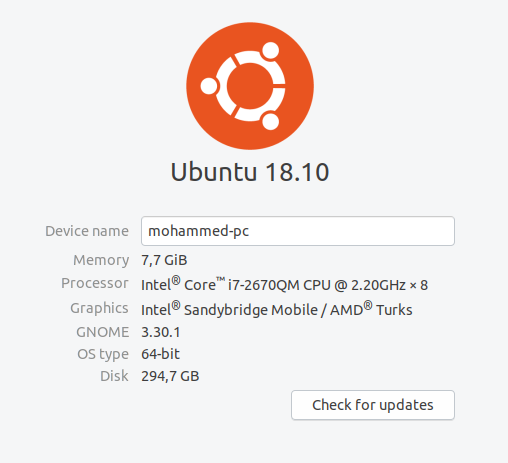
\includegraphics[scale=0.3]{009_os}
\captionsetup{justification=centering}
\caption{To be edited}
\end{figure}

\begin{figure}[h!]
\centering
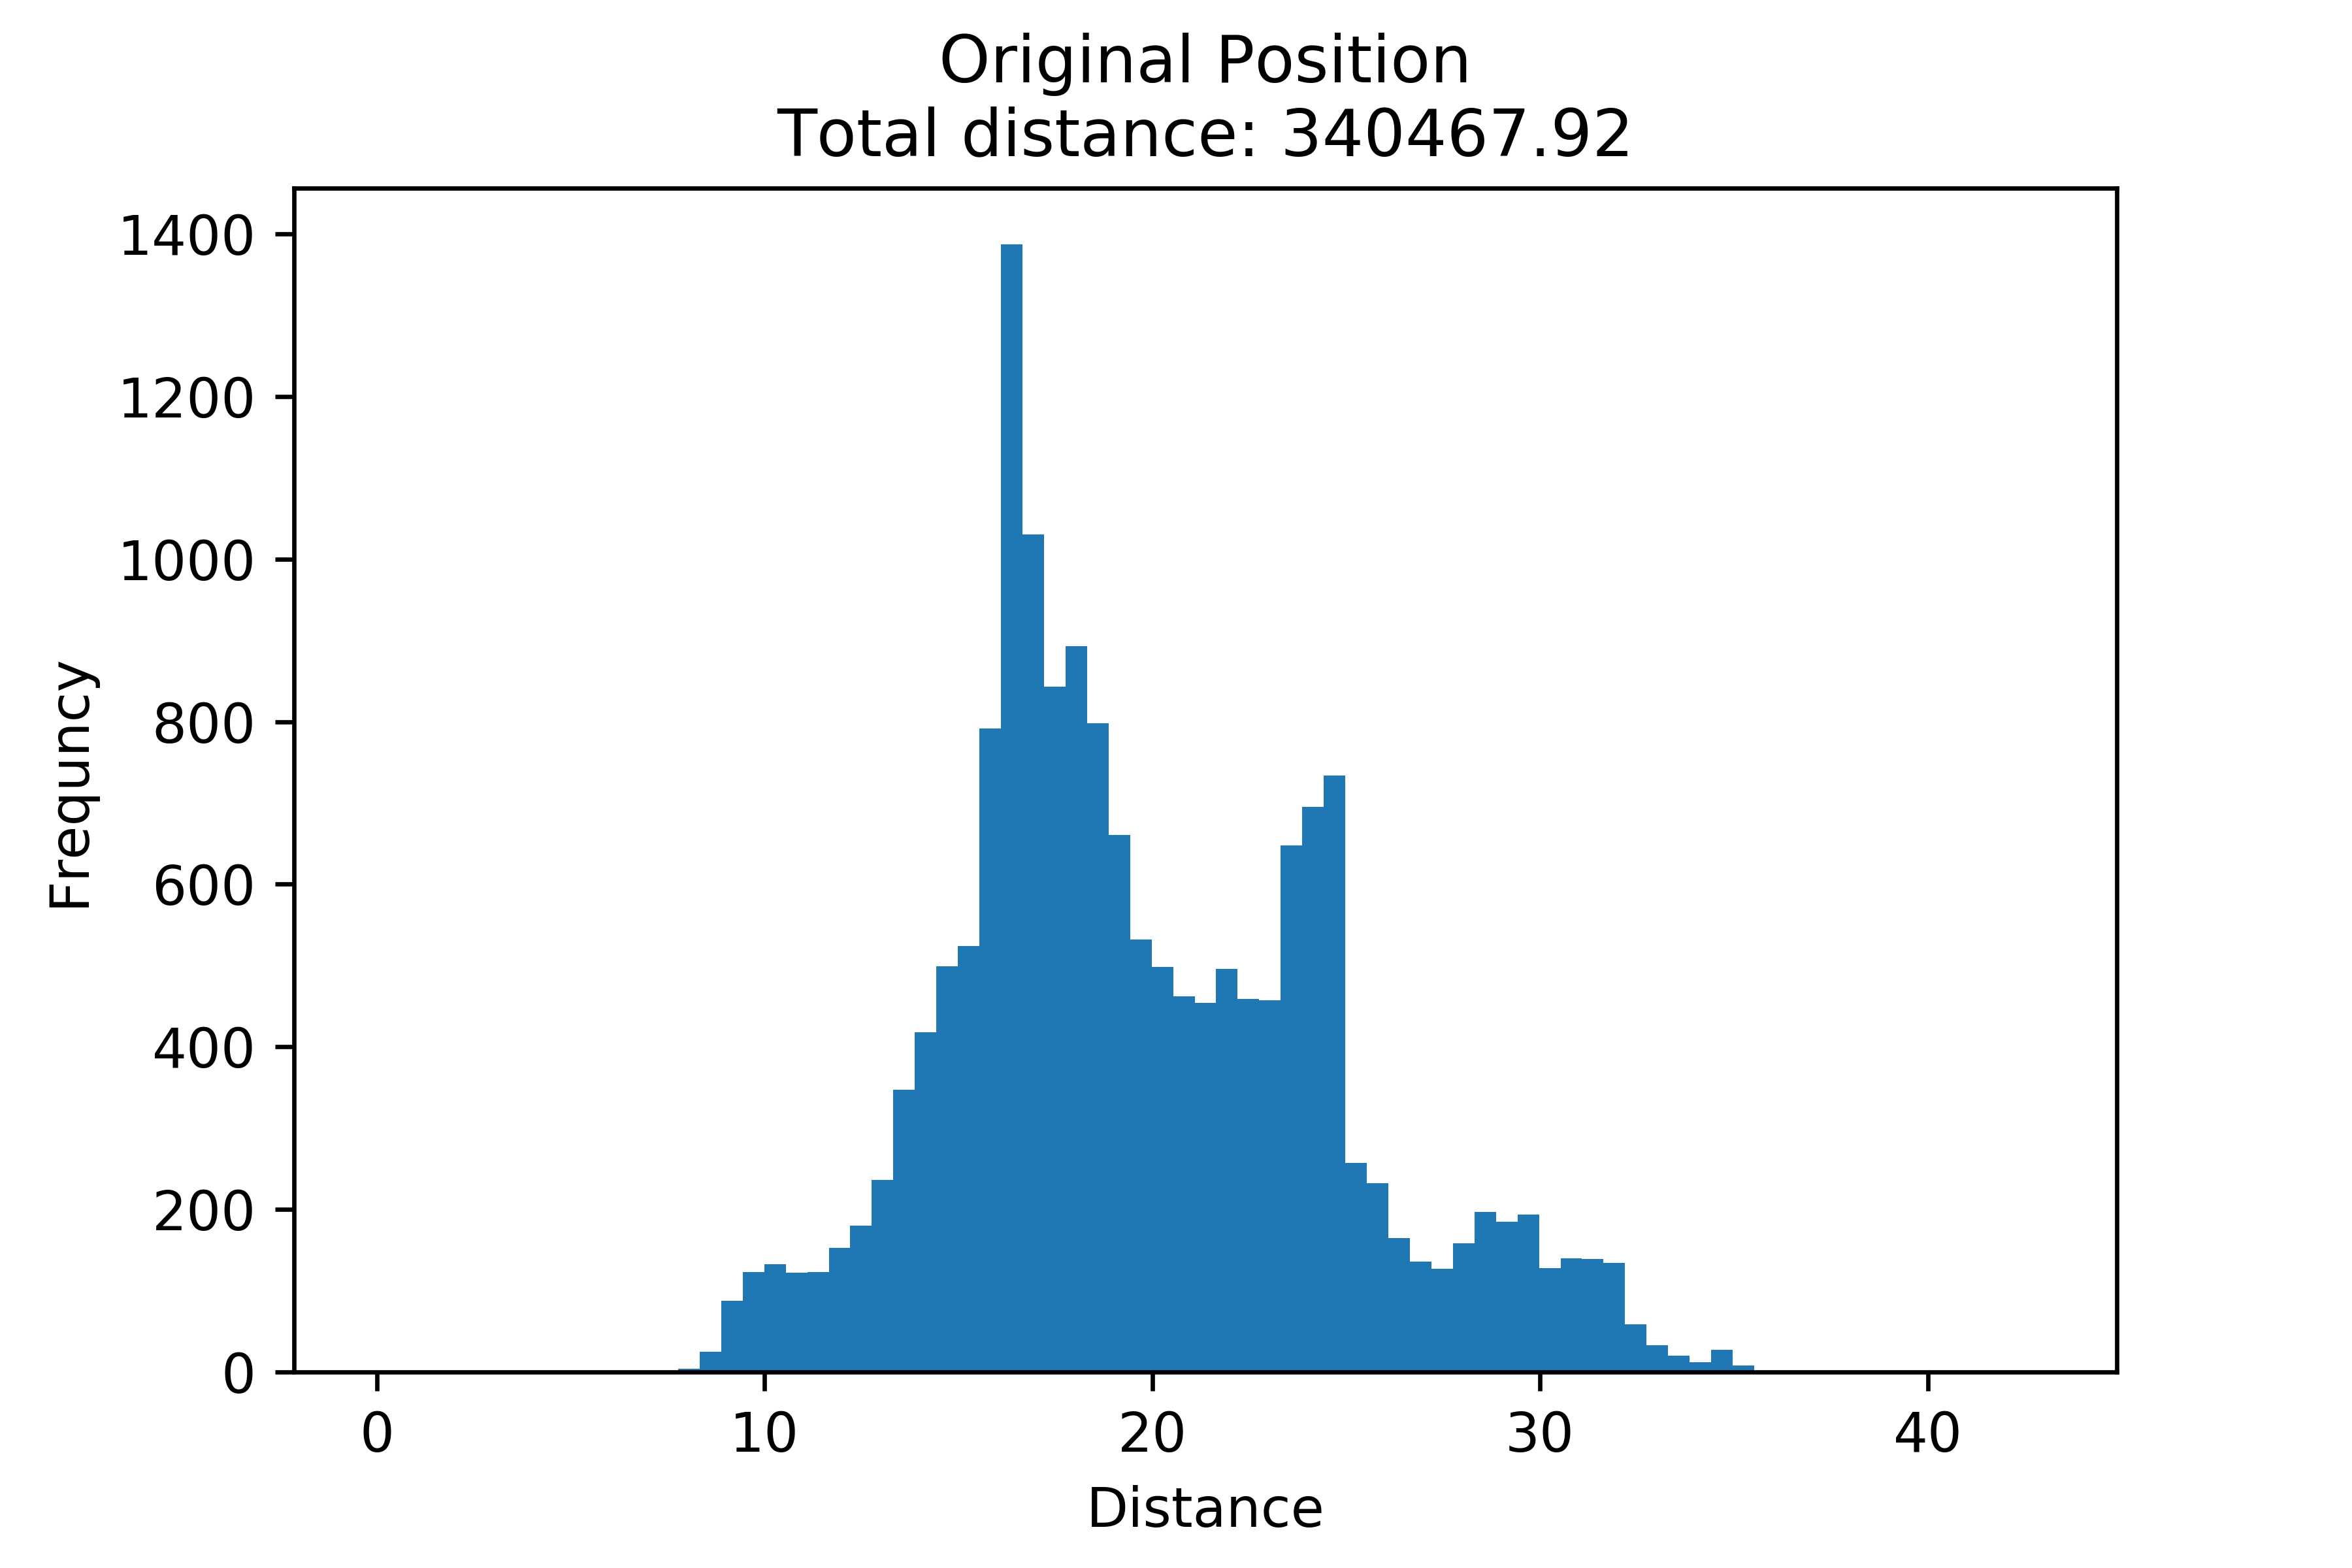
\includegraphics[scale=1]{010_hist_original}
\captionsetup{justification=centering}
\caption{To be edited}
\end{figure}


\begin{figure}[h!]
\centering
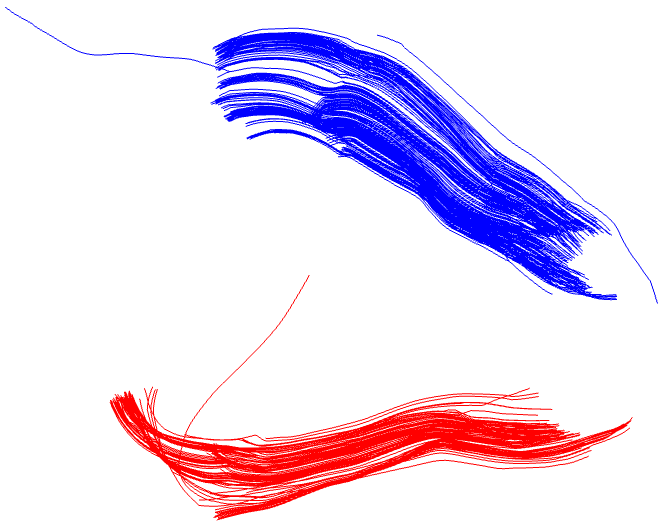
\includegraphics[scale=0.5]{011_img_original}
\captionsetup{justification=centering}
\caption{To be edited}
\end{figure}

\begin{figure}[h!]
\centering
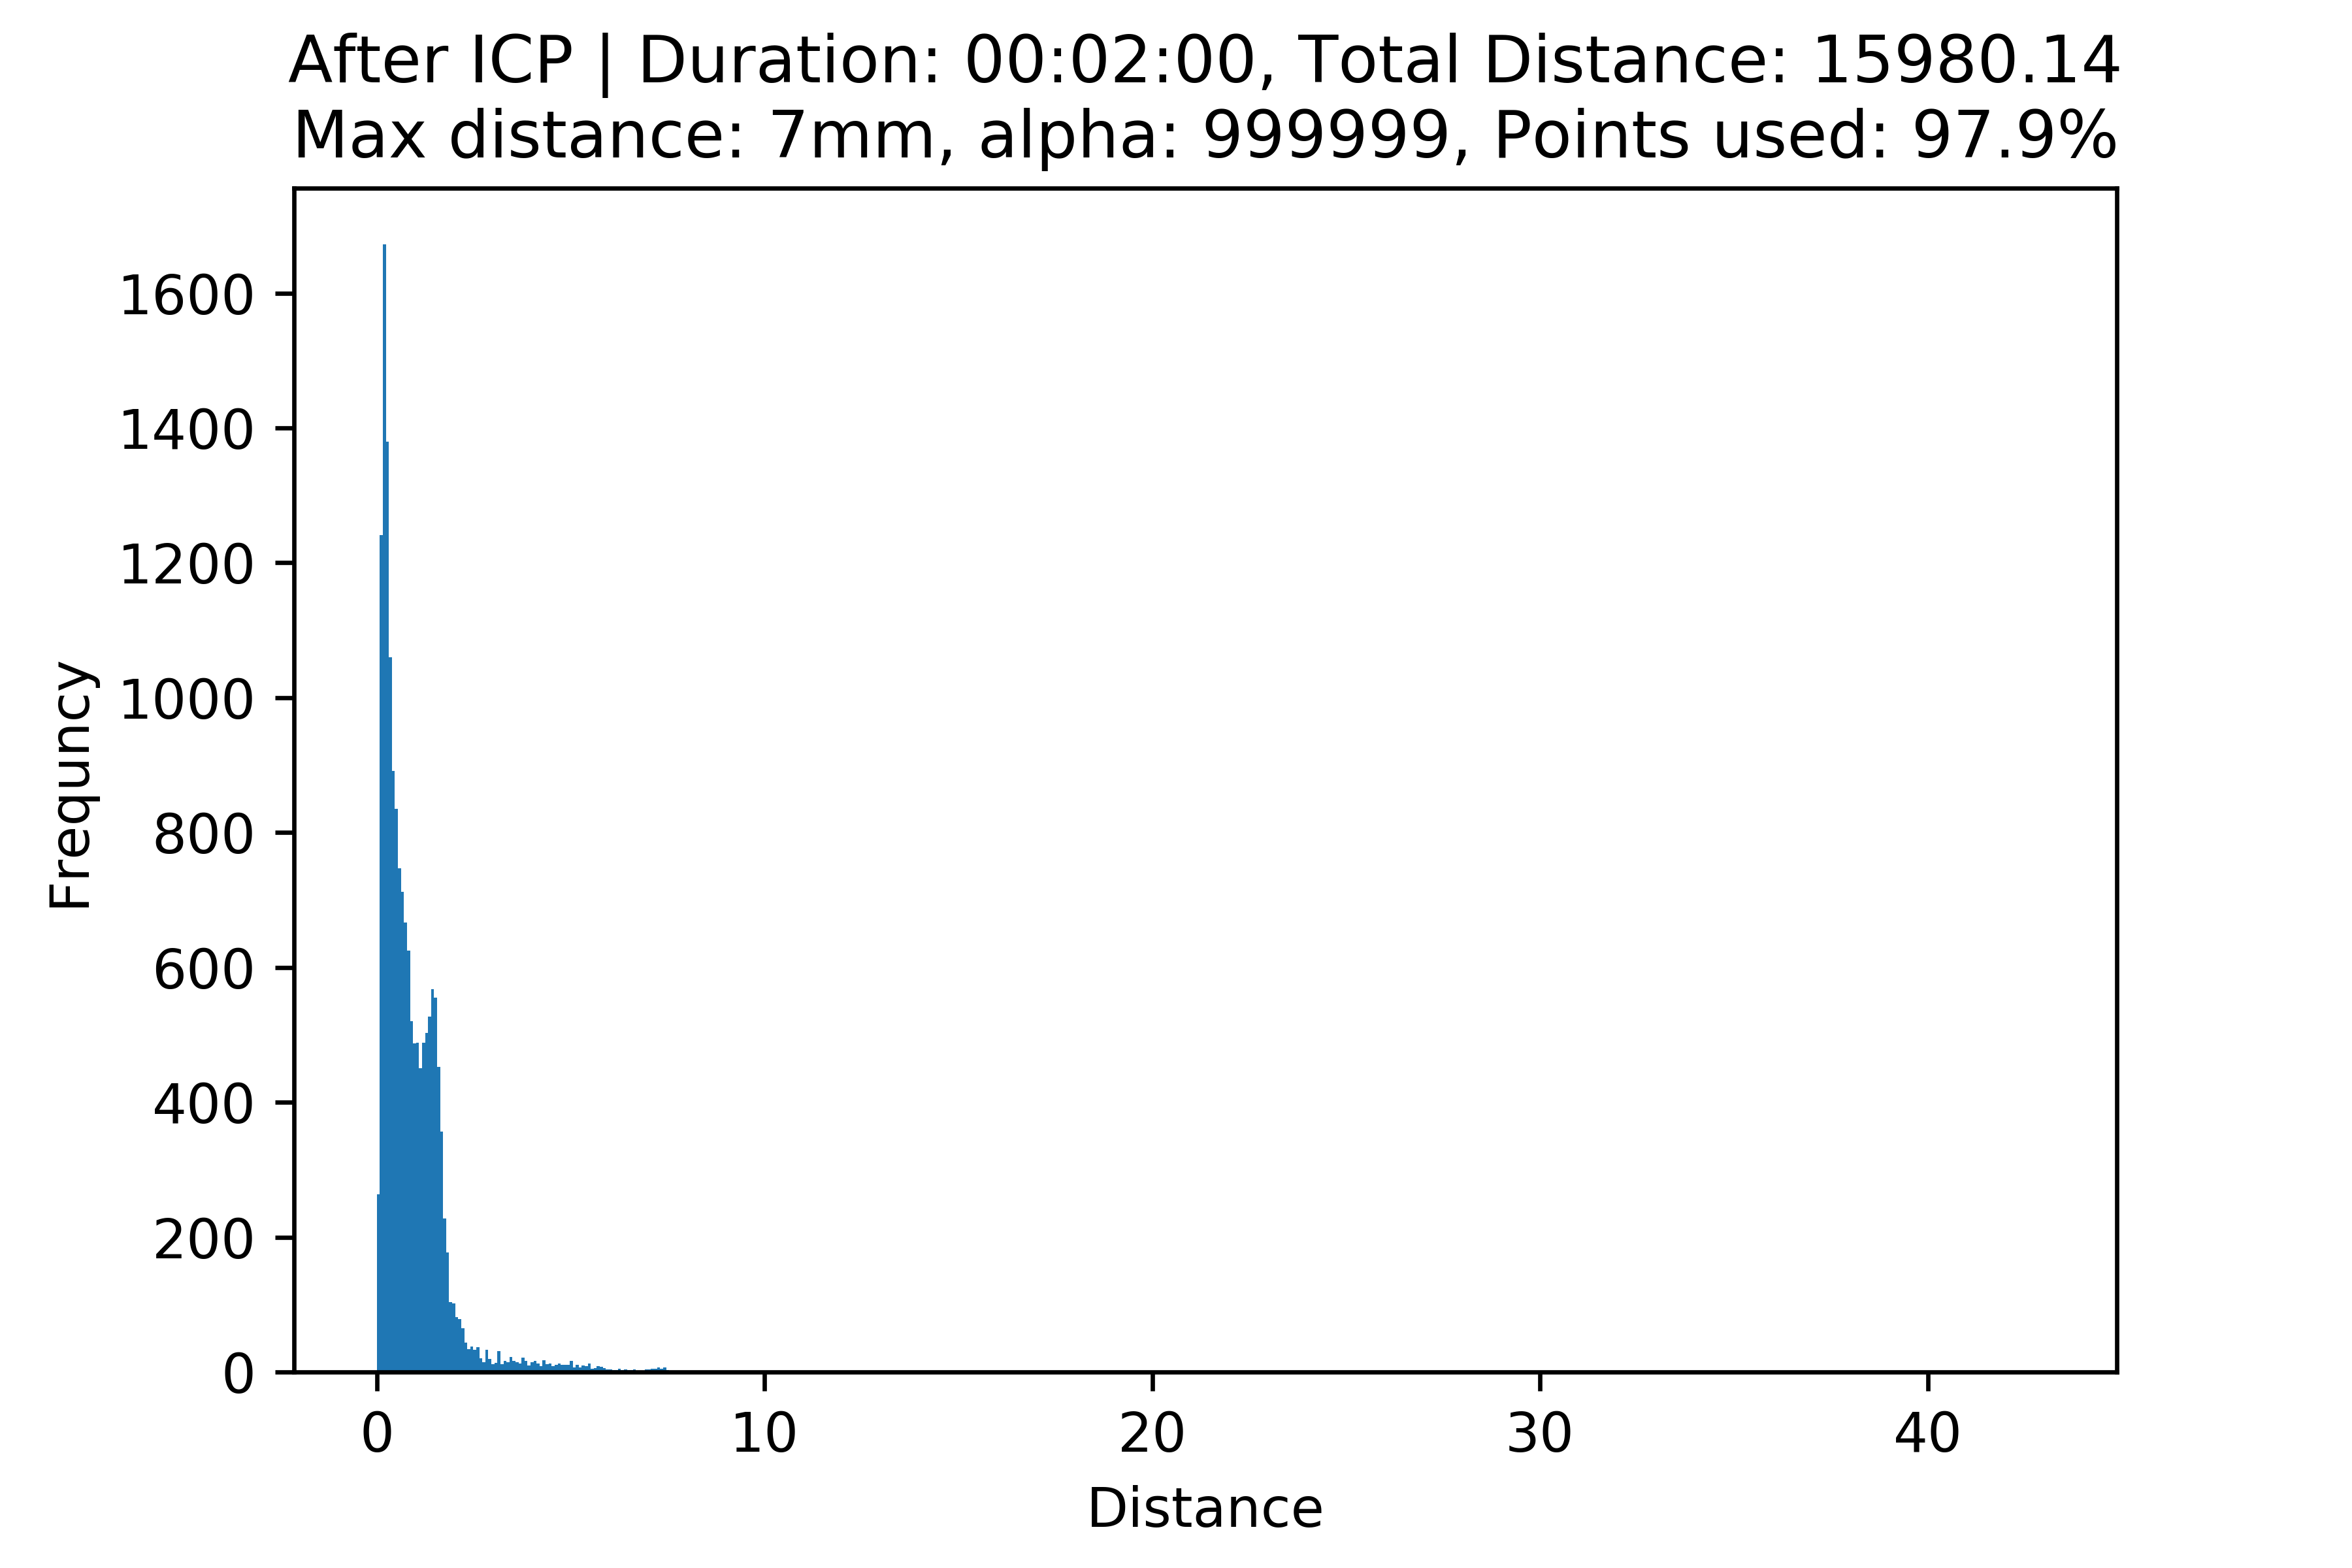
\includegraphics[scale=1]{012_hist_ICP}
\captionsetup{justification=centering}
\caption{To be edited}
\end{figure}

\begin{figure}[h!]
\centering
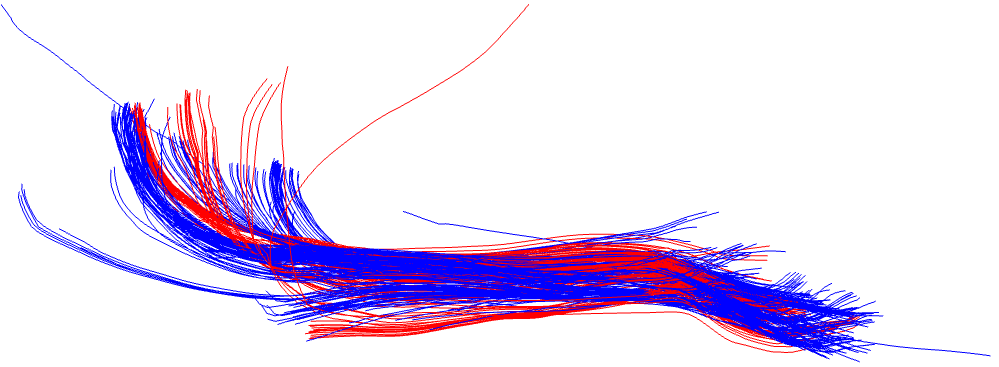
\includegraphics[scale=0.4]{013_img_ICP.png}
\captionsetup{justification=centering}
\caption{To be edited}
\end{figure}

\begin{figure}[h!]
\centering
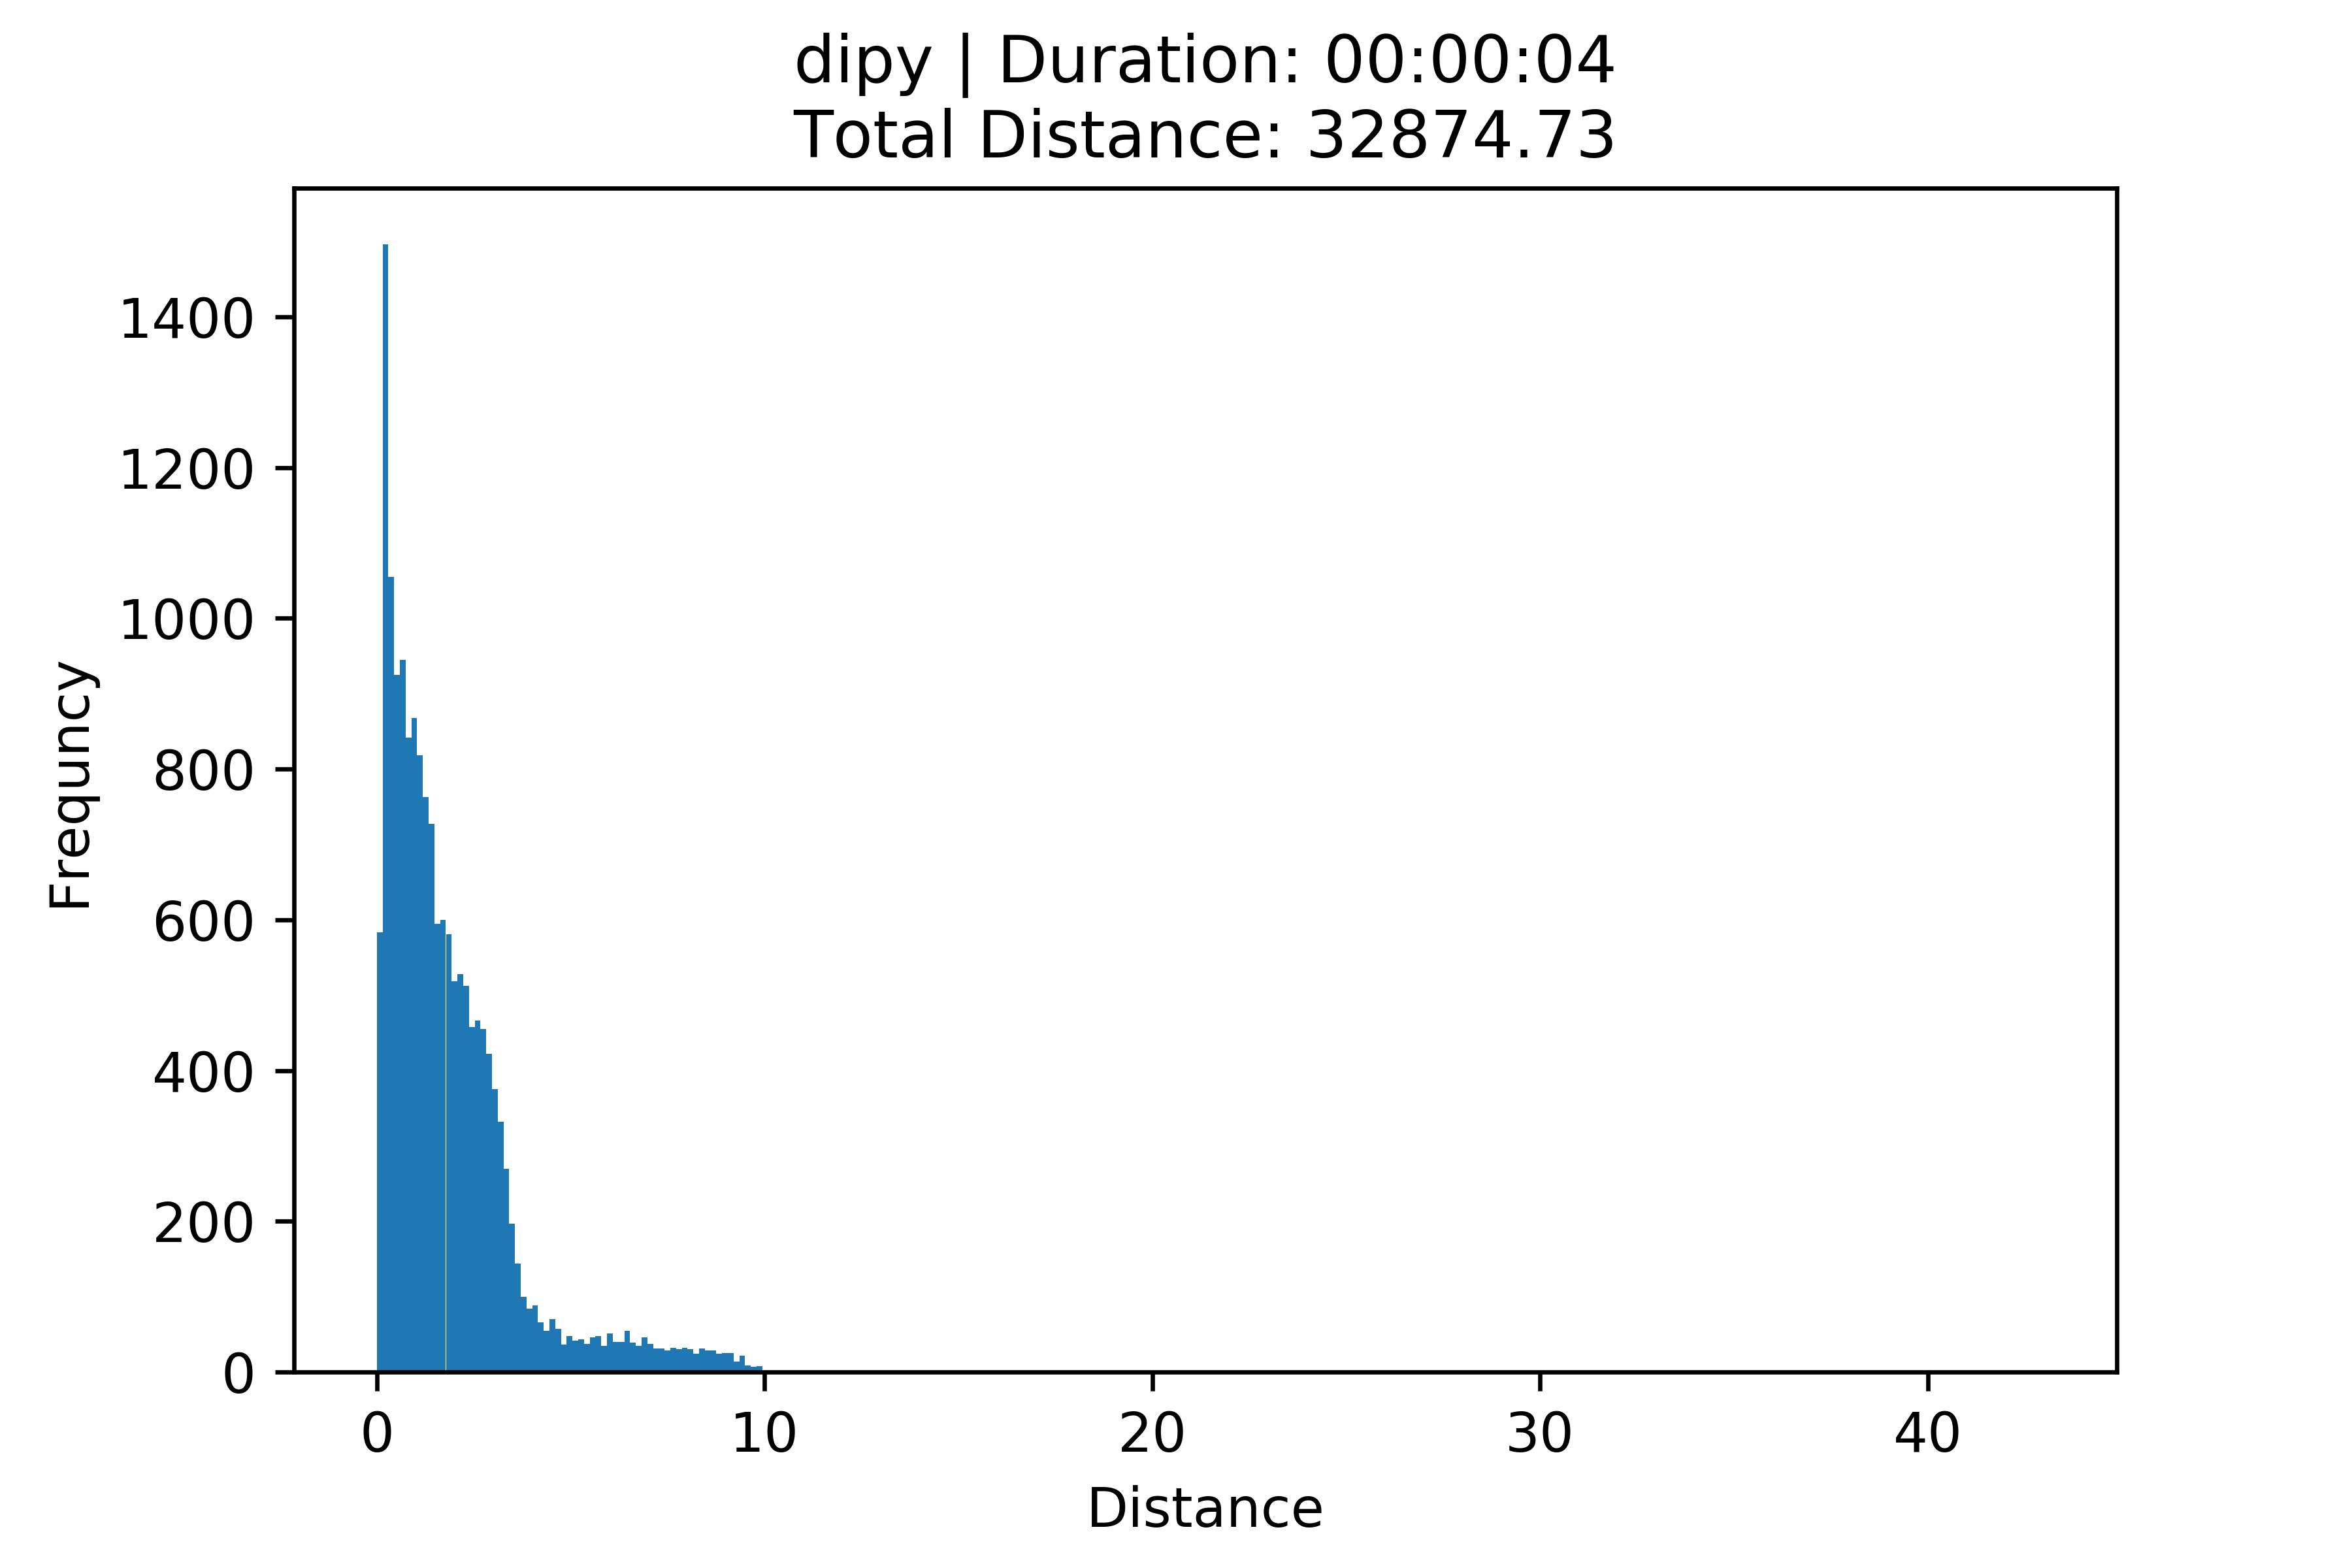
\includegraphics[scale=1]{014_dipy_hist}
\captionsetup{justification=centering}
\caption{To be edited}
\end{figure}

\begin{figure}[h!]
\centering
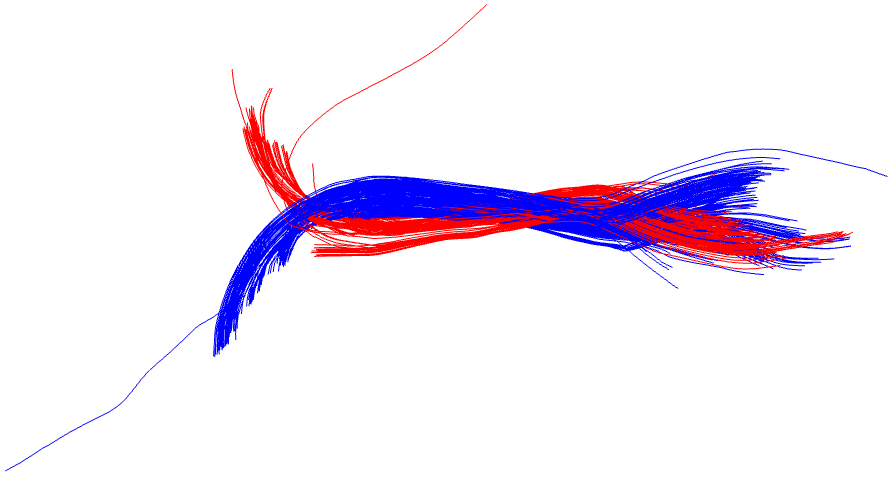
\includegraphics[scale=0.5]{015_img_dipy}
\captionsetup{justification=centering}
\caption{To be edited}
\end{figure}

\begin{figure}[h!]
\centering
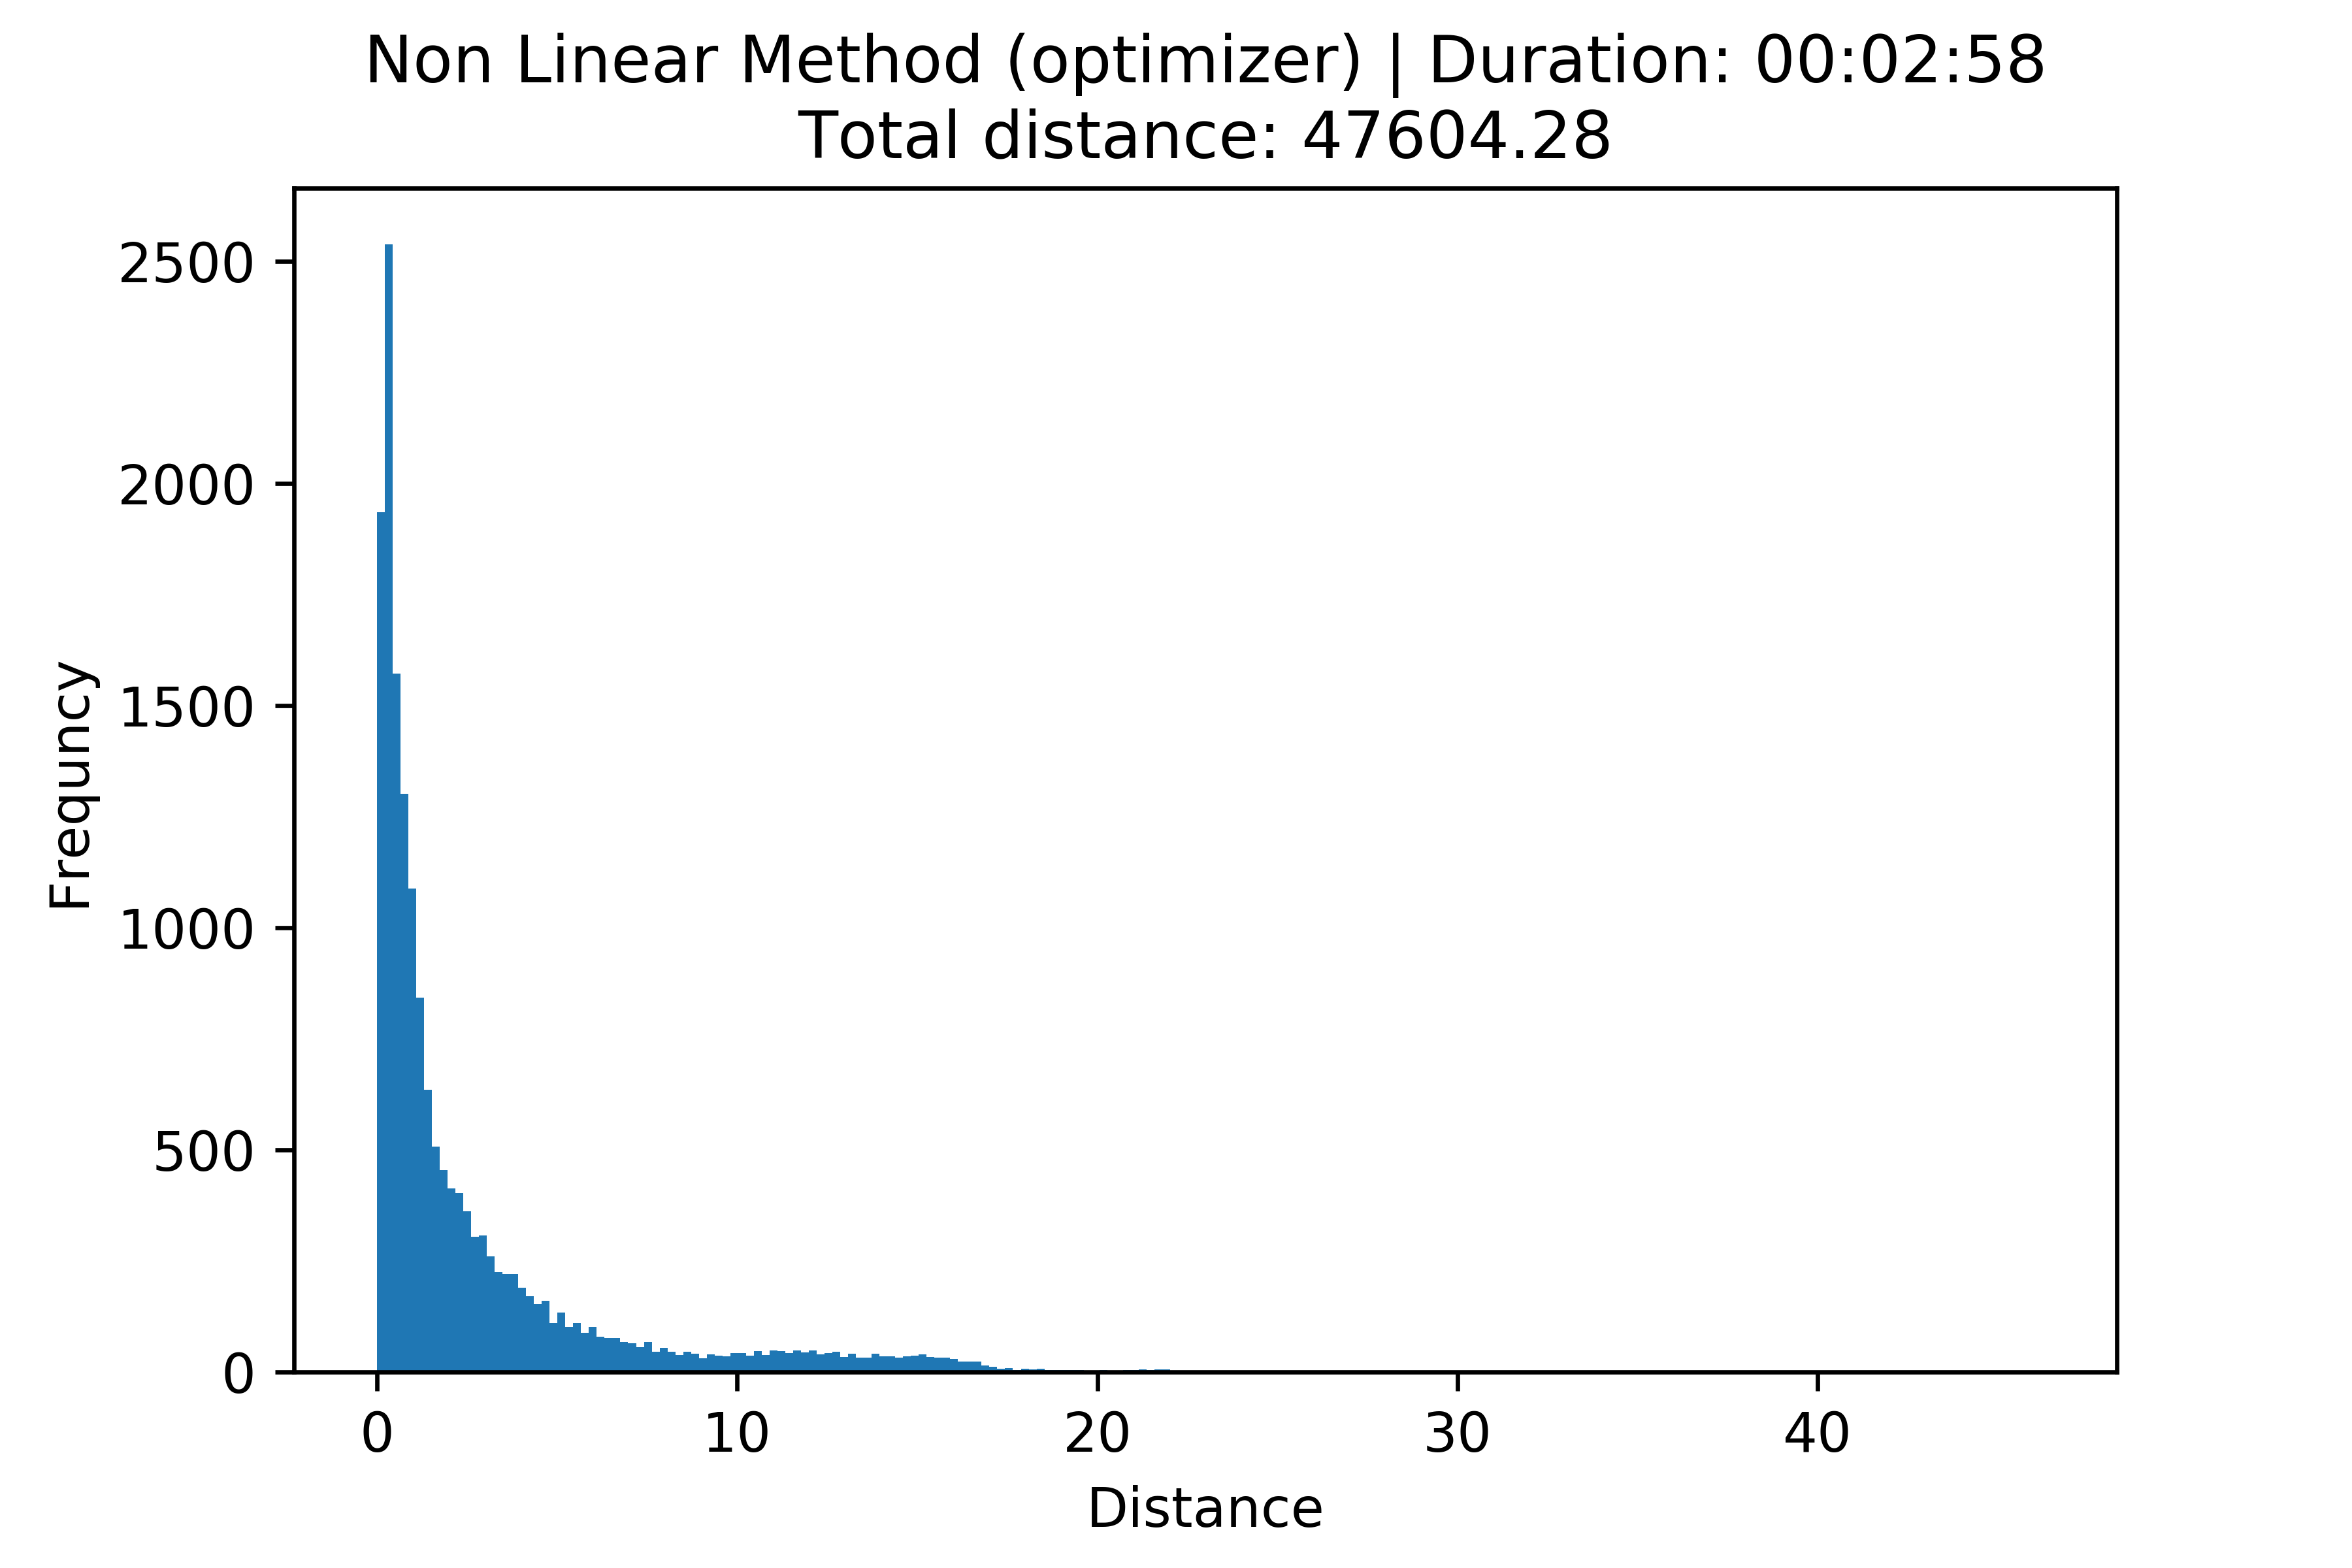
\includegraphics[scale=1]{016_hist_nonlinear}
\captionsetup{justification=centering}
\caption{To be edited}
\end{figure}

\begin{figure}[h!]
\centering
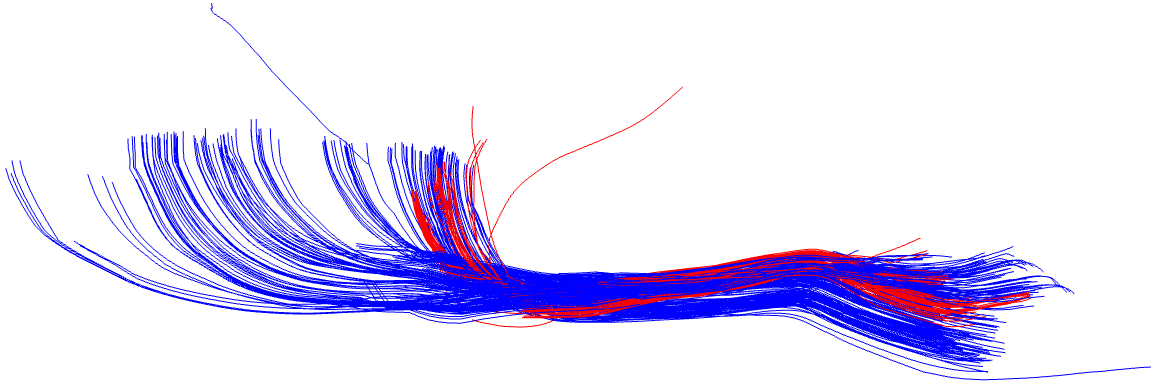
\includegraphics[scale=0.4]{017_img_non_linear}
\captionsetup{justification=centering}
\caption{To be edited}
\end{figure}

\end{document}